\chapter{Introdução}

A organização mundial da saúde (OMS) projeta que a depressão será a principal causa de incapacidade em 2030, impondo gastos à saúde superiores à doença cardíaca isquêmica (OMS, 2008). A depressão é um fator de risco para o início e progressão de incapacidade física e social. Além disso, indivíduos com depressão ou demais psicopatologias podem desenvolver outras condições de saúde mais cedo, devido a fatores comportamentais e biológicos correlacionados à doença. \cite{Nestler2013}

Muitos pacientes afetados por transtornos de humor e ansiedade são estigmatizados. É uma doença que possui maior impacto nos níveis de incapacidade do que nos de mortalidade. Todavia, mais pesquisas vem colaborando para o aumento na compreensão das bases científicas desses transtornos. \cite{Kandel} A depressão é uma doença crônica, e quando não tratada, aumenta-se a probabilidade da recorrência de um episódio depressivo no futuro. A depressão é uma das principais causas de suicídio e está associada a várias condições médicas, como obesidade, diabetes, acidente vascular cerebral, doença de Parkinson e esclerose múltipla, além de um maior risco de doença de Alzheimer e morte súbita cardíaca. \cite{Nestler2006} Entre $10\%$ e $20\%$ da população mundial terá um episódio grave (ou seja, clinicamente significativo) ao longo da vida. Depressão e outras manifestações afetivas graves podem representar até $50\%$ de hospitalizações por razões psiquiátricas. \cite{Cooper2003}

\begin{figure}[H]
\centering
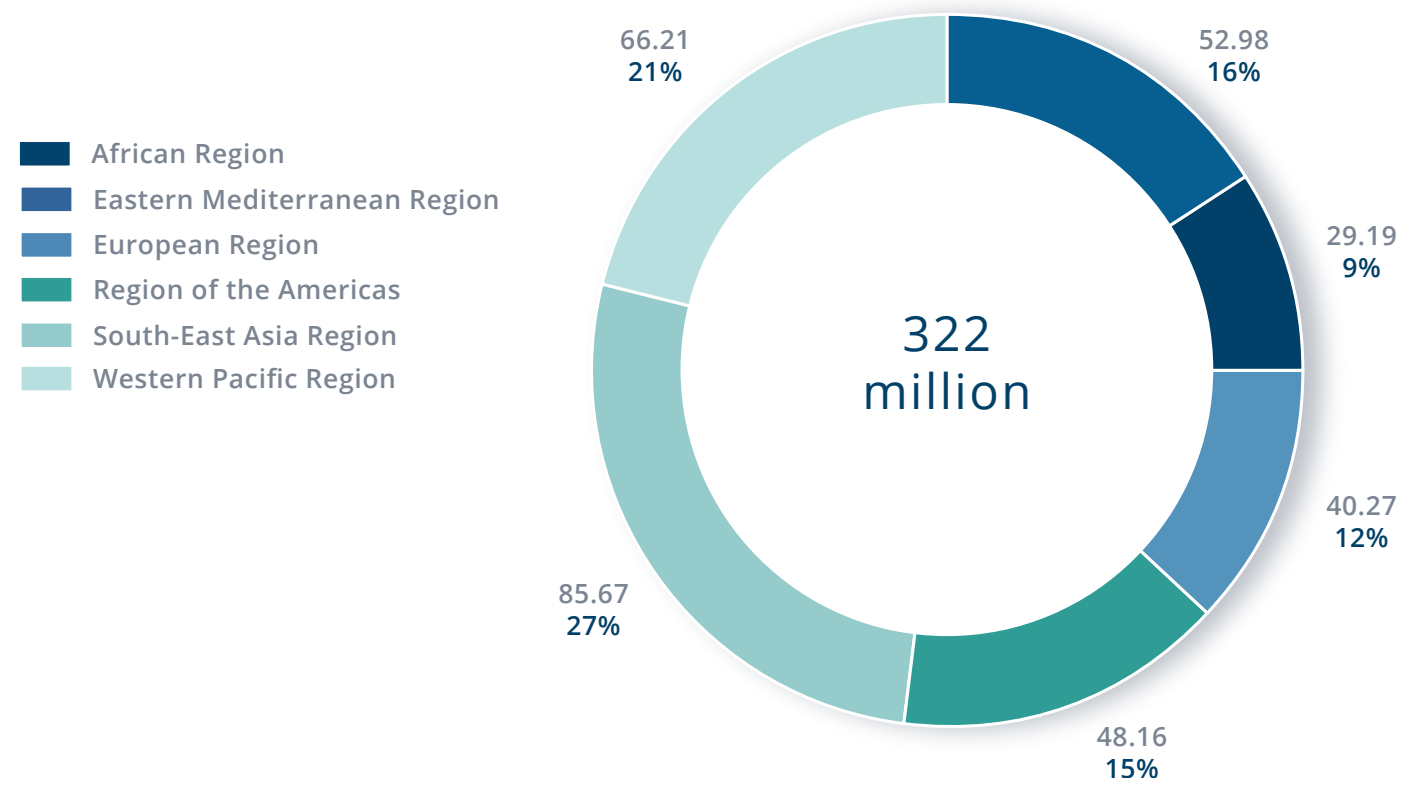
\includegraphics[scale=1]{Figuras/who2017.png}
\caption{Gráfico destacando a ocorrência do transtorno depressivo em 2015 que atingiu $4,4\%$ da população mundial.  \cite{WHO2017}}
\end{figure}

 É um complexo transtorno psiquiátrico que afeta $\approx 15\%$ da população mundial, tendo um enorme custo social. Embora acredite-se que seja resultado de interações gene-ambiente, os genes causadores e os fatores ambientais subjacentes à depressão ainda são desconhecidos. Os medicamentos antidepressivos atualmente em uso, cujo precursor foi descoberto por acaso em meados de 1950, modulam a neurotransmissão por monoamina e levam de seis a oito semanas para exercer seus efeitos, mas cada medicamento é eficaz em apenas $60 - 70\%$ dos pacientes. \cite{Wong2004} 

Há uma crescente percepção de que, longe de ser uma doença com manifestações puramente psicológicas, a depressão maior é uma doença sistêmica com efeitos em diversos sistemas do organismo. \cite{Charney2004}

Eventos estressantes da vida têm uma associação causal substancial com a depressão, e agora há evidências convincentes de que mesmo o estresse no início da vida constitui um fator de risco importante para o desenvolvimento subsequente da depressão. \cite{Charney2004}

Embora muitos agentes psicofarmacológicos estejam atualmente
disponíveis para o tratamento da depressão, uma porcentagem grande de pacientes de $20 - 30\%$ tratados com antidepressivos comumente usados não alcançam recuperação completa e desenvolvem uma resistência ao tratamento. A razão mais associada a esse distúrbio incapacitante é que a depressão é uma desordem multifacetada com causas diversas, desde fatores moleculares até culturais, mostrando que nosso conhecimento sobre seus mecanismos patogenéticos ainda é muito limitado. \cite{Kim} 

A grande maioria dos antidepressivos disponibilizados atualmente, são oriundos da hipótese monoaminérgica publicada há mais de 60 anos. Na prática clínica tem-se que $\approx 50\%$ dos pacientes apresentam remissão completa. \cite{Nestler2006} 

Nem idade, gênero ou grupo social é imune à depressão clínica. Muitos pacientes ainda são relutantes em procurar ajuda devido ao estigma associado à depressão e demais transtornos psiquiátricos. \cite{Jane2017} As causas subjacentes da maioria dos transtornos de humor e ansiedade permanecem desconhecidas. Há um forte componente hereditário nas doenças psiquiátricas que, quando associadas às influências ambientais, resultam em maior vulnerabilidade. \cite{Nemeroff2005} Aproximadamente $40-50\%$ do risco de depressão pode ser herdado, embora os genes específicos subjacentes ainda não foram identificados até o momento. \cite{Nestler2006}

Foram feitos esforços intensivos de pesquisa para melhor caracterizar os fundamentos genéticos e bioquímicos das doenças mentais. No entanto, a maioria dos transtornos psiquiátricos, incluindo transtornos de humor e ansiedade, são de natureza poligênica, em vez de determinados unicamente pela genética mendeliana autossômica tradicional. As evidências de estudos pré-clínicos, epidemiológicos e clínicos convergiram para demonstrar de forma convincente que eventos estressantes ou traumáticos que ocorrem no início da vida aumentam significativamente o risco de depressão e outras doenças psiquiátricas na idade adulta. Os circuitos neurais contendo fator de liberação de corticotrofina (CRF) foram identificados como um importante mediador da resposta ao estresse. A adversidade no início da vida resulta em mudanças críticas na resposta ao estresse e um risco muito maior de depressão em pessoas geneticamente predispostas. \cite{Nemeroff2005}

Emoções são respostas transitórias a um estímulo específico no ambiente. Quando um estado emocional é prolongado e torna-se dominante ao longo do tempo, constitui-se humor. Sendo assim, o humor pode ser independente das circunstâncias pessoais ou ambientais. Os transtornos de humor geralmente envolvem depressão ou euforia. Os transtornos de ansiedade envolvem a regulação anormal do medo.  \cite{Kandel}

Em ambos os transtornos, os sintomas principais possuem um componente emocional fundamental, além de serem acompanhados por alterações fisiológicas, cognitivas e comportamentais. Ambos envolvem estados emocionais negativos e parecem abranger circuitos neurais que incluem a amígdala e o córtex cingulado anterior. Isso talvez possa explicar o porquê de aproximadamente $60\%$ dos pacientes com depressão maior, também sofrerem de transtorno de ansiedade. Em grande parte dos casos, transtornos de ansiedade precedem o início de sintomas depressivos. \cite{Kandel}

\section{Epidemiologia e correlação sociodemográfica}

Conforme o DSM-5, estima-se que 7\% da população nos Estados Unidos é acometida pelo transtorno depressivo, com prevalência na faixa etária entre 18-29 anos, sendo 3 vezes mais frequente comparada a pessoas acima de 60 anos. Além disso, ainda não se tem a explicação do porquê mulheres tendem a possuir 1,5-3 vezes maior taxa de algum episódio depressivo ao longo da vida. \cite{DSM5}

A depressão maior ocorre duas vezes mais frequentemente entre mulheres. A razão para essa diferença entre gêneros é
desconhecida. Explicações especulativas incluem disparidades hormonais, fatores de personalidade, fatores sociais ou ambientais e exposição a eventos estressantes da vida. Por outro lado, a prevalência de depressão é revertida entre as crianças, onde os meninos possuem maiores taxas. A mudança surge durante a adolescência e continua ao longo da vida adulta. \cite{DSM5}

\section{Distinção entre tristeza e um episódio depressivo}




